\section{NP-nehéz feladatok polinomiális esetei, additív és multiplikativ hiba}

\begin{description}
	\item[Független élhalmaznak] nevezzük a gráf éleinek egy olyan halmazát
	      amelyben semelyik két élnek nincs közös pontja -- $\nu(G)$ jelöli a legnagyobb
	      független élhalmaz elemszámát.
	\item[Független ponthalmaz]  a csúcsók olyan részhalmaza amelyik semelyik két
	      pont nincs közös élen -- $\alpha(G)$ jelöli a legnagyobb független ponthalmaz
	      elemszámát.
	\item[Lefogó ponthalmaz] a gráf pontjainak egy halmaza amely a gráf minden
	      élének legalább egyik végét tartalmazza -- $\tau(G)$ a legkisebb lefogó
	      ponthalmaz elemszáma.
	\item[Lefogó élhalmaz] az élek egy halmaza, ha a gráf minden pontjára legalább
	      egy elem illeszkedik -- $\rho(G)$ a legkisebb lefogó élhalmaz elemszáma.
	\item[Gallai tétel] $\forall~G$ gráf ahol a gráf: \begin{itemize}
		      \item hurokmentes $\Rightarrow \tau(G)+\alpha(G) = |V(G)|$.
		      \item izoláltpont mentes $\Rightarrow \nu(G) +\rho(G) = |V(G)|$.
	      \end{itemize}
	\item[König tétel] $\forall~G$ gráf ahol a gráf: \begin{itemize}
		      \item páros $\Rightarrow \tau(G)=\nu(G)$,
		      \item izoláltpont mentes $\Rightarrow \rho(G) = \alpha(G)$,
	      \end{itemize}
	      és a magyar módszer megtalálja mind a négy halmazt.
	\item[König tétel] $G=(A,B,E)$ páros gráfban $\Rightarrow \chi_e(G) =
		      \Delta(G)$, azaz az élkromatikus szám~\footnote{A gráf élkromatikus száma
		      $k$, ha a gráf élei $k$  színnel kiszínezhető, úgy, hogy $\forall~2$
		      szomszédos él különböző színű. } megegyezik a maximális fokszámmal.
\end{description}

Az utóbbi bizonyítása az algoritmus megadásával történik, mely segítségével
bármely $G$ páros gráfban $\Delta(G)$ darab színnel az élek kiszínezhetőek;
hatékonyan, nagy méretű gráfra is. Jelölje $G$ éleit $E=\{ e_i \}$, ahol legyen
$|E|=m$. Az algoritmus egymás után színezi az éleket $\Delta(G)$ szín valamelyikével.
Eközben előfordul, hogy szint kell cserélni egy élen, de azt színtelené tenni nem.

Tegyük fel, hogy $e_1, \cdots, e_{i-1}$ már ki van színezve és legyen
$e_i=\{u,v\}$, ahol $u \in A$ és $v \in B$. $u$ és $v$ csúcsra is legfeljebb
$\Delta(G)$ él illeszkedik, de ezek közül $e_i$ még biztos, hogy színtelen.
Tehát mindkét csúcsban van még legalább egy szabad szín (olyan színű él oda még
nem kapcsolódik). Ha ez a szín azonos $u$ és $v$--ben akkor használjuk azt, és
készen vagyunk $e_i$--vel.

Ha a szín nem közös, akkor tegyük fel, hogy $u$ szabad színe piros, míg $v$
szabad színe kék. Legyen $C$ a $G$ gráf azon részgráfja amely felveszi $G$
összes csúcsát, de az élek közül csak a piros vagy kék színűeket. $C$
részgráfban minden minden pont foka legfeljebb $2$ (hiszen minden csúcsra
legfeljebb egy piros és egy kék illeszkedhet). Ekkor $C$ diszjunkt utakból és
körökből épül fel.

Ugyanakkor $u$ és $v$ csúcs foka $C$--ben csak egy lehet hiszen $u$--nak piros,
$v$--nek kék a szabad színe. Ezért $u$ és $v$ is egy $C$--beli út végpontja.
Legyen $P_u$ az út melynek végpontja $u$. $v$ nincs rajta ezen, mert másképp az
út másik végpontja pont $v$ lenne. Ekkor $P_u$ páratlan sok élből állna, hiszen
a gráf páros, az egyik osztályból indul ($A$) és másikban ér véget ($B$).

Tehát $P_u$--nak az élei váltakozó színűek, kezdete kék, tehát az utolsó él is
kék színű kell, hogy legyen. Így $P_u$ végpontja nem lehet $v$, mert arra nem
illeszkedik kék él. Fessük át $P_u$ kék éleit pirosra és piros éleit kékre.
Ezzel a színezést nem rontjuk el, de most $u$--nak kék lett a szabad színe. Most
már $u$ szabad színe megegyezik $v \not \in P_u$ szabad színével (kék),
színezzük meg ezzel az $e_i$ élet és megvagyunk.

\subsection{Probléma osztályok}
\begin{description}
	\item[P] a polinomiális időben megoldható problémák.
	\item[NP] azon eldöntési problémák amelyre létezik az igen válaszra tanú.
	\item[co--NP] azon eldöntési problémák amelyre létezik a nem válaszra tanú.
	\item[NP--nehéz] $\forall$ NP--beli probléma visszavezethető az ilyen problémára.
\end{description}

\begin{figure}[htbp]
	\caption{Probléma osztályok}
	\label{fig:ProbOszt}
	\centering
	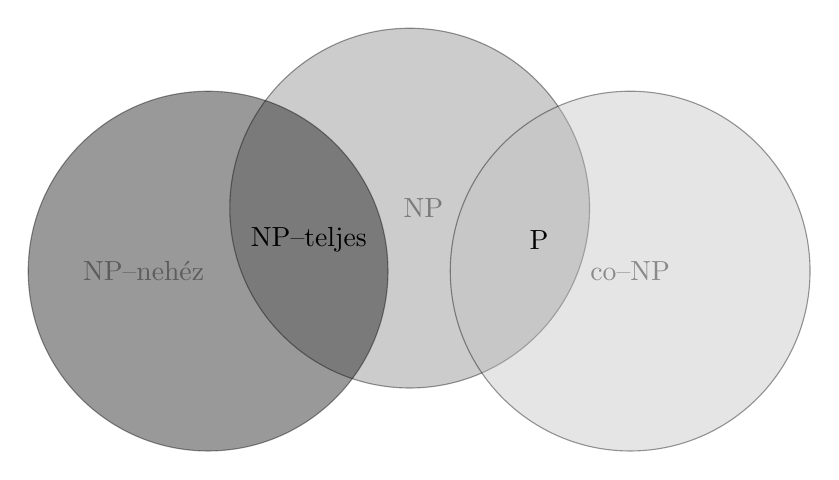
\begin{tikzpicture}[scale=0.8]
		\tikzset{venn circle/.style={draw,circle,minimum width=6,fill=#1,opacity=0.4}}
		\node [venn circle = gray,minimum width=130] (NP) at (0,0) {~~~NP};
		\node [venn circle = lightgray,minimum width=130] (coNP) at (3.5,-1) {co--NP};
		\node [venn circle = black,minimum width=130] (NPn) at (-3.2,-1) {NP--nehéz~~~~~~~~~~~~~~~};
		\node[] at (barycentric cs:NP=1/2,NPn=1/2 ) {NP--teljes};
		\node[right] at (barycentric cs:NP=1/2,coNP=1/2 ) {P};
	\end{tikzpicture}
\end{figure}

\Aref{fig:ProbOszt} ábra mutatja a probléma osztályok közötti relációkat, nyílt
kérdés, hogy $P=NP$ fen áll e vagy sem.

\begin{table}
	\begin{tabular}{|m{6.5cm}|m{2cm}|m{3.5cm}|}
		\hline
		Feladat                                                         & Probléma   & Algoritmus                             \\
		\hline\arrayrulecolor{lightgray}
		Összefüggőség                                                   & P          & mélységi bejárás és szélességi bejárás \\  \hline
		$\exists$ ? teljes párosítás gráfban                            & P          & javító utak                            \\\hline
		$\exists$ ? $2$ színezés gráfban                                & P          & mélységi bejárás                       \\\hline
		$\exists$ ? $3$ színezés gráfban                                & NP--teljes &                                        \\\hline
		síkba rajzolhatóság                                             & P          & Kuratowski--tétel                      \\\hline
		klikk                                                           & NP--nehéz  &                                        \\\hline
		MAXFTL                                                          & NP--nehéz  &                                        \\\hline
		MAXFTL páros gráfban                                            & P          & magyar--módszer                        \\\hline
		Hamilton kör                                                    & NP--teljes &                                        \\\hline
		utazó ügynők problémája                                         & NP--nehéz  &                                        \\\hline
		maximális élszámú vágás keresése                                & NP--nehéz  &                                        \\\hline
		maximális élszámú vágás keresése, ha a hálózat síkba rajzolható & NP--nehéz  &                                        \\\hline
		$\alpha(G), \tau(G), \chi(G), \chi_e(G)$                        & NP--nehéz  &                                        \\\hline
		$\alpha(G), \tau(G), \chi(G), \chi_e(G)$ ha G páros             & P          &                                        \\\hline
		leghosszabb irányított út                                       & NP--nehéz  &                                        \\\hline
		leghosszabb irányított út páros gráfban                         & P          & mélységi bejárás                       \\
		\hline
	\end{tabular}
\end{table}

\subsection{Additív hiba}

Legyen egy $f(X)$ minimalizálandó célfüggvény $X_I$ halmazon, amely $I$ bemeneten
értelmezett. Egy algoritmus $c$ additív hibával közelítve old meg egy minimalizálási
problémát, ha bármely $I$--re polinom időben ad egy $y_I \in X_I$ megoldást, amire teljesül, hogy:

\[
	f(y_I) \leq \underbrace{(\mbox{min}_{X \in X_I} f(X))}_{\mbox{optimum}} +
	\underbrace{c}_{\mbox{hiba}}.
\]

Például  határozzuk meg egy $G$ gráfban (amelybe nincs hurokél, többszörös él és
irányított él) az \emph{élkromatikus számot}. Ekkor tudjuk, hogy $\Delta(G)=k$ és a
Vizing tétel~\footnote{A Vizing-tétel alsó és felső korlátot ad egy egyszerű
	gráf élkromatikus számára. A tételt Vagyim Georgijevics Vizing 1964--ben
	bizonyította be. A tétel szerint egy egyszerű gráf élkromatikus száma legfeljebb
	eggyel nagyobb a maximális fokszámánál, azaz ha a gráf minden csúcsában k-nál
	kevesebb él találkozik, akkor ki tudjuk színezni az éleit legfeljebb k színnel:
	$\Delta(G) \leq \chi_e(G) \leq \Delta(G)+1.$}
alapján az élkromatikus szám $k$ vagy $k+1$. Hogy melyik azt
eldönteni egy NP--teljes feladat, de a tétel bizonyítása alapján polinom időben
megkapható egy $k+1$ színezés, azaz $1$ additív hibájú az algoritmus.

Egy másik példa a \emph{kromatikus szám} (színezés) keresése egy gráfban. Az öt szín
tétel alapján polinomiális időben beszínezhető bármely gráf. Tehát egy adott
síkgráfon az optimális színezés legyen $1$ ha az üres, $2$ ha az páros, és $5$
másképpen. E utolsó esetben $\chi(G) \geq 3$, tehát a hiba $\leq 2$.

De például egy gráfban a \emph{leghosszabb út megkeresésének} problémája (amely
NP-teljes, hiszen a Hamilton-út keresését magába foglalja) semmilyen additív $c$
konstanssal közelítő algoritmussal nem oldható meg (ha csak P$=$NP nem
teljesül).

Ennek belátásához tegyük fel, hogy lenne egy olyan $A_c$ algoritmus, amely
tetszőleges $G$ gráfbaban megadna egy olyan kört, amelynek hossza legfeljebb
$c$--vel kisebb a leghosszabb út hosszánál. Osszuk fel $G$ minden élét $c$ darab
új ponttal, és a kapott gráfot jelöljük $H$--val. Beláthatjuk, hogy:
\[ H\mbox{--ban leghosszab kör hossza} = (c+1) \cdot G\mbox{--ben leghosszab
		kör hossza} \]

Tehát, $H$--ban leghosszab kör hossza egy $c+1$--el osztható egész szám.  Most
futassuk le $A_c$ algoritmust $H$--ra, és a kapott eredményt kerekitsük fel a
legközelebbi $c+1$--el osztható számhoz. Ezzel megadtuk $H$--beli maximális kör
hosszát, és innen $G$--beli is kifejezhető. Ez egy hatékony algoritmus lenne
pontos leghosszabb út megkeresésére. De ennek létezése elentmond annak, hogy a
feladatt NP--nehéz, tehát indirekt bizonyitottuk állitásunk.

\subsection{Multiplikatív hiba}

Egy algoritmus $k>1$ multiplikatív hibával közelítve old meg egy minimalizálási
problémát, ha $\forall~I$ bemenetre polinom időben ad egy $y_I \in X_I$
megoldást amire:


\[
	f(y_I) \leq \underbrace{k}_{\mbox{hiba}}  \cdot \underbrace{(\mbox{min}_{X \in X_I} f(X))}_{\mbox{optimum}}.
\]

Például keressük egy $G$ gráfban a \emph{minimális lefogó ponthalmazt} ($\tau(G)$).
Válasszuk ki a független élek maximális rendszerét ($\nu$), mindkét végpontját
tekintve egy $2\nu$ elemű ponthalmazt kapunk. Definíció szerint legfeljebb annyi
független él választható ki, mint a lefogó pontok minimális száma ($\nu \leq
	\tau$), tehát egy $k=2$ multiplikatív hibával rendelkező algoritmusról van szó.

A \emph{maximális páros részgráf} megállapításához keressük az $n$ pontú gráf olyan
szétosztását, ahol a két pontosztály között a legtöbb él halad. Ez a feladat egy
NP--nehéz probléma. Induljunk ki egy tetszőleges kettéosztásból és, ha egy pont
áthelyezése növeli a vágás élszámát akkor azt helyezzük át.

E naiv algoritmus a maximális vágás legalább felét kiadja, tehát ez is egy $k=2$
multiplikatív hibával rendelkező algoritmus. Az algoritmus lépésszám becslése
$\mbox{max}_k\{k\cdot(n-k)\}\approx \dfrac{n^2}{4}$, ami polinom idejű, tehát teljesíti
a követelményeket.
